\section{funzioni trigonometriche}
\label{sec:funzioni_trigonometriche}%
\label{sec:avvolgimento}%

Consideriamo la circonferenza unitaria 
\[
  U = \ENCLOSE{z\in \CC\colon \abs{z} = 1}.
\]
Ogni punto $z\in U$ individua un angolo geometrico con l'asse reale.
Il nostro obiettivo è ora quello di definire la misura di un angolo.
Il punto $z=1$ individuerà un angolo di misura nulla e 
ruotando $z$ in senso antiorario vogliamo ottenere angoli 
di misura crescente in modo che l'angolo che si ottiene 
giustapponendo uno di seguito all'altro gli angoli individuati 
dal punto $z$ e dal punto $w$ abbia misura pari alla somma delle misure 
degli angoli individuati da $z$ e da $w$.

Scegliamo arbitrariamente di dare una misura $\tau>0$ all'angolo giro.
L'idea intuitiva è quella di \emph{arrotolare} la retta $\RR$ come un filo 
attorno alla circonferenza $U\subset \CC$ 
mandando il punto $0\in \RR$ sul punto $1\in \CC$,
e poi il punto $\frac \tau 4$ su $i$, il punto $\frac \tau 2$ su $-1$,
il punto $3\frac \tau 4$ su $-i$ e il punto $\tau$ di nuovo su $1$.
Punti intermedi andranno su punti intermedi di $U$ in modo da avere 
l'additività degli angoli: la misura della somma di due angoli dovrà 
essere la somma delle misure.

L'insieme $U$ eredita la struttura di gruppo moltiplicativo di $\CC$: 
se $z,w\in U$ 
allora $z\cdot w \in U$ in quanto $\abs{z\cdot w} = \abs{z}\cdot \abs{w} = 1$
essendo $\abs{z}=\abs{w}=1$.
Ricordiamo inoltre che la moltiplicazione di numeri complessi unitari 
corrisponde alla somma dei loro angoli geometrici.
Dunque la funzione $\phi\colon \RR \to U$ che misura gli angoli, 
dovrà avere la proprietà di \emph{omomorfismo}:
\begin{equation}\label{eq:4012387}
  \phi(x+y) = \phi(x)\cdot \phi(y).
\end{equation}
Purtroppo sul gruppo $U$ non possiamo mettere un ordinamento e 
dunque non possiamo utilizzare il teorema~\ref{th:isomorfismo} 
di isomorfismo 
come abbiamo fatto per definire la funzione esponenziale.
L'idea sarà invece quella di definire la funzione $\phi$ 
bisezionando l'angolo giro, quindi estendendola ai multipli 
degli angoli bisecati con \eqref{eq:4012387}
e, infine, estendendola per monotonia a tutti gli angoli.

\begin{theorem}
\label{th:omomorfismo_U}
Fissato $\tau>0$ esiste una unica funzione $\phi\colon \RR \to \CC$ 
tale che 
\begin{enumerate}
\item $\abs{\phi(t)}=1$,
\item $\phi(t+s)=\phi(t)\cdot \phi(s)$ (proprietà di omomorfismo),
\item $\phi(\tau) = 1$ e $\phi(t)\neq 1$ per ogni $t\in(0,\tau)$,
\item $\Im\phi(t)$ è crescente per $t\in\Enclose{0,\frac \tau 4}$.
\end{enumerate}

Inoltre tale funzione ha le seguenti proprietà:
\begin{enumerate}
  \item $\phi(t+\tau)=\phi(t)$ ($\phi$ è $\tau$-periodica),
  \item $\phi([0,\tau)) = U = \ENCLOSE{z\in \CC\colon \abs{z}=1}$,
  \item $\Im \phi(t)\colon \Enclose{0,\frac \tau 4}\to [0,1]$
  è strettamente crescente e bigettiva,
\end{enumerate}
\end{theorem}
%
\begin{proof}
Per fissare le idee facciamo la costruzione con $\tau=4$ 
cioè decidiamo di voler dare misura $1$ all'angolo retto e 
quindi misura $4$ all'angolo 
giro. 
E' facile osservare che se riusciamo a costruire $\phi$ con le proprietà 
richieste per $\tau=4$ allora la funzione $t\mapsto \phi(\tau t / 4)$ 
avrà le proprietà richieste per un $\tau$ generico.

Avendo scelto $\tau=4$ si ha $1 = \phi(4) = \phi(2)^2$. 
Dunque $\phi(2)=-1$ (esercizio~\ref{ex:radice_uno}, 
ricordiamo che $\abs{\phi(t)}=1$ e che $t=4$ 
è il primo punto in cui $\phi$ vale $1$).
Ora si ha $\phi(1)^2=-1$ e dunque $\phi(1)=\pm i$ (esercizio~\ref{ex:radice_quarta_uno}).
Visto che $\Im \phi$ è richiesto sia crescente in $[0,1]$ dovrà essere
$\phi(1)=i$. 
Sarà dunque sufficiente definire $\phi$ sull'intervallo $[0,1]$, 
perché poi si avrà $\phi(t+1)=\phi(t)\cdot \phi(1) = i\phi(t)$
e dunque $\phi(t+k)=i^k\phi(t)$ per ogni $k\in \ZZ$.

La funzione $\phi\colon[0,1]\to U$
associa alla misura $t\in[0,1]$ l'angolo rappresentato da 
un numero complesso unitario $z=\phi(t)\in U$ con $\Re z\ge 0$ e $\Im z\ge 0$
(nel primo quadrante del piano complesso) in modo tale 
che l'angolo retto, rappresentato da $i\in \CC$, abbia misura $1$: $\phi(1)=i$.

Per fare questo dobbiamo innanzitutto bisecare un generico angolo 
$u\in U$.
Se $u\in U$ l'angolo metà è rappresentato da un numero 
complesso $z\in U$ tale che $z^2=u$. 
L'equazione $z^2=u$ ha in generale due soluzioni (si veda l'esercizio~\ref{ex:radice_complessa}), 
ma se $u$ 
è nel primo quadrante $Q=\ENCLOSE{z\in U\colon \Re z\ge 0, \Im z\ge 0}$
ci sarà una sola soluzione nel primo quadrante.
Posto $u=a+ib$ e $z=x+iy$ si avrà (esercizio~\ref{ex:radice_complessa})
\[
  x = \sqrt{\frac{1+a}{2}}, \qquad 
  y = \sqrt{\frac{1-a}{2}}.
\]
Denotiamo con $z=\sqrt u$ la soluzione con parte reale positiva 
dell'equazione $z^2=u$ che abbiamo appena calcolato.
Possiamo allora definire la successione degli angoli dimezzati:
\[
\begin{cases}
u_0 = i\\
u_{n+1} = \sqrt{u_n}.
\end{cases}
\]
Moralmente $u_n = \sqrt[2^n] i$.
Questi angoli sono uno la metà dell'altro $u_{n+1}^2 = u_n$.
Induttivamente si dimostra facilmente che vale $u_{n+k}^{2^k} = u_n$
per ogni $n,k\in \NN$.

Avendo posto $\tau=4$ dovrà essere $\phi(1)=i$ e quindi 
$\phi(1/2^n)=u_n$ affinchè sia rispettata l'equazione \eqref{eq:4012387}.
Inoltre dovrà essere
\begin{equation}
\phi\enclose{\frac{p}{2^n}} = (u_n)^p,
\qquad n\in \NN, p\in \NN, p\le 2^n.
\end{equation}
Questa definizione è ben posta in quanto se $\frac{p}{2^n}=\frac{q}{2^{n+k}}$
si ha $q=2^k p$ e quindi 
$(u_n)^p = (u_{n+1})^{2p} = \dots = (u_{n+k})^{2^k p} = 
u_{n+k}^q$.

Posto 
\[
B = \ENCLOSE{\frac{p}{2^n}\colon n\in \NN, p\in \NN, p\le 2^n} \subset [0,1]
\]
abbiamo definito $\phi\colon B\to U$ in modo che \eqref{eq:4012387}
sia soddisfatta. 
Inoltre la definizione di $\phi$ è unica se imponiamo  
$\phi(1)=i$.
Si tratta ora di estendere la definizione di $\phi$ a tutto 
l'intervallo $[0,1]$. 
Puntiamo ad utilizzare il teorema~\ref{th:estensione_monotona} di 
estensione monotona.

Innanzitutto vogliamo dimostrare che $\Re \phi\colon B\to \RR$ 
e $\Im \phi\colon B\to \RR$ sono funzioni monotone.
In particolare vogliamo dimostrare che se $t\ge s$ allora 
$\Re \phi(t) \le \Re \phi(s)$.
Osserviamo che si ha $\phi(t) = \phi(s)\cdot \phi(t-s)$, 
quindi basta capire come si comporta la moltiplicazione per un 
numero complesso del primo quadrante.
Se $\phi(s)=z=a+ib$ e $\phi(t-s)=w=x+iy$ si ha
$\Re (zw) = ax-by$. 
Banalmente se $a,b,x,y\in[0,1]$ si ha $ax-by \le a$. 
Dunque $\Re \phi(t)\le \Re \phi(s)$ come volevamo dimostrare.
Visto che $\Im \phi(t) = \sqrt{1-\Re \phi(t)^2}$ si ha
anche $\Im \phi(t) \le \Im \phi(s)$.

Questa proprietà ci dice in particolare che $\phi$ assume valori 
nel primo quadrante, in quanto sapendo che agli estremi 
$\phi(0) = 1$ 
e $\phi(1)=i$ ogni altro valore deve avere parte reale 
e parte immaginaria compresa tra $0$ e $1$.

Possiamo allora considerare la funzione 
$f=\Im \phi$, $f\colon B\subset [0,1]\to[0,1]$
a cui applicare il teorema~\ref{th:estensione_monotona}.
Dobbiamo verificare che $f(B)$ è denso in $J=[0,1]$. 
Dati $y_1,y_2\in [0,1]$ con $y_1<y_2$ dobbiamo mostrare che esiste $t\in B$ tale 
che $y_1 < \Im \phi(t) < y_2$.
Sarà $y_1=\Im z_1$ e $y_2=\Im z_2$ con $z_1,z_2\in U$.
L'idea è quella di considerare $n$ abbastanza grande in modo tale 
che i punti $f(p/2^n)= \Im \phi(p/2^n)$ siano abbastanza ravvicinati tra loro.

Ci servirà dimostrare che per ogni $n\ge 1$ si ha
\begin{equation}
  \label{eq:44385834}
  \abs{u_n-1}^2 \le \frac{2}{2^n}.
\end{equation}
La disequazione~\eqref{eq:44385834} si dimostra per induzione.
Per $n=1$ si nota che 
$u_1=\frac{1+i}{\sqrt 2}$ (esercizio~\ref{ex:bisezione}) e quindi,
$\abs{u_1-1}^2 = \dots = 2-\sqrt 2 \le 1$ e dunque 
\eqref{eq:44385834} è soddisfatta.
Per il passo induttivo è sufficiente dimostrare che:
\begin{equation}
  \label{eq:4398633}
   \abs{u_{n+1}-1}^2 \le \frac 1 2 \abs{u_n-1}^2.
\end{equation}
E infatti si ha
\[
  \abs{u_n-1}^2
  = \abs{u_{n+1}^2-1}^2
  = \abs{u_{n+1}-1}^2 \abs{u_{n+1}+1}^2
\]
e, osservando che $\Re u_{n+1}\ge \Re u_1 = 1/\sqrt 2$ si ha
\[
 \abs{u_{n+1}+1}^2 \ge \Re^2(u_{n+1}+1) 
 \ge \enclose{\frac{1}{\sqrt 2}+1}^2 = \frac 1 2 + \sqrt 2 + 1 > 2.
\]
Questo conclude la dimostrazione di~\eqref{eq:4398633} e 
quindi anche di~\eqref{eq:44385834}.

Grazie a \eqref{eq:4398633} possiamo scegliere $n$ abbastanza grande in modo che 
$\abs{u_n-1}<y_2-y_1$. 
Questo significa che per ogni $p\in \NN$, $p\le 2^n$ si ha 
\[
  0
  \le f\enclose{\frac{p+1}{2^n}} - f\enclose{\frac{p}{2^n}}
  = \Im u_n^{p+1} - \Im u_n^p 
  \le \abs{u_n^{p+1}-u_n^p}
  = \abs{u_n}^p \abs{u_n-1} 
  = \abs{u_n-1} \le y_2-y_1.
\]
Dunque deve esistere $p$ per cui $f(p/2^n)$ sta tra $y_1$ e $y_2$.
Questo dimostra che $f(B)$ è denso in $[0,1]$.

Per il teorema~\ref{th:estensione_monotona} possiamo allora estendere 
$f$ in modo unico ad una funzione crescente $\tilde f \colon [0,1]\to [0,1]$.
Ma allora possiamo estendere anche $\phi$ a tutto $[0,1]$,
in modo unico,
ponendo $\phi(t) = \sqrt{1-{\tilde f}^2(t)} + i \tilde f(t)$. 
In questo modo $\Im \phi = \tilde f$ è monotona crescente mentre 
$\Re \phi=\sqrt{1-{\tilde f}^2}$ risulta decrescente.

Vogliamo ora dimostrare che la funzione $\tilde f\colon [0,1]\to [0,1]$ 
è bigettiva.
Innanzitutto $\tilde f$ è strettamente crescente (oltre che crescente)
perché se fosse $\tilde f(t_1)=\tilde f(t_2)$ con $t_1<t_2$ esisterebbero 
$s_1,s_2\in B$ con $t_1<s_1<s_2<t_2$ tali che $\tilde f(s_1)=\tilde f(s_2)$.
E questo non è possibile perché $\tilde f(s_1)=f(s_1)$ e $\tilde f(s_2) = f(s_2)$ sono potenze 
diverse di uno stesso $u_n$. Dunque $\tilde f$ è iniettiva.
Sia ora $C=\tilde f([0,1])$ l'immagine di $\tilde f$. 
Ovviamente $\tilde f\colon [0,1]\to C$ è suriettiva e quindi bigettiva.
La funzione inversa $g\colon C \to [0,1]$ soddisfa anch'essa 
le ipotesi del teorema~\ref{th:estensione_monotona}
(ovviamente $g(C)=[0,1]$ è denso in $[0,1]$ e si osserva che 
$0\in C$ e $1\in C$).
Dunque se fosse $C \neq [0,1]$ si potrebbe estendere $g$ a tutto
$[0,1]$ mantenendo la monotonia. 
Ma visto che $g$ assumeva già tutti i valori di $[0,1]$ significa 
che l'estensione di $g$ non è più iniettiva.
Esistono cioè $y_1<y_2$ tali che $g(y_1)=g(y_2)=x$
e visto che $g$ è monotona si avrà $g(y)=x$ per ogni $y\in[y_1,y_2]$. 
Ma l'immagine della funzione $\tilde f$ 
contiene al più un punto di tale intervallo, e questo è assurdo 
perché l'immagine di $\tilde f$ contiene l'immagine di $f$ che 
è densa in $[0,1]$.
Dunque $f = \Im \phi\colon[0,1]\to[0,1]$ è bigettiva e strettamente 
crescente.

Vogliamo ora verificare che la proprietà di omomorfismo 
\eqref{eq:4012387} è verificata su $[0,1]$.
Prendiamo dunque $s,t\in[0,1]$ tali che anche $s+t\in [0,1]$
e puntiamo a dimostrare che per ogni $\eps>0$ 
si ha:
\begin{equation}\label{eq:4438844}
  \Im(\phi(s+t)- \phi(s)\phi(t)) < 4\eps,
  \qquad
  \Re(\phi(s+t)-\phi(s)\phi(t)) < 4\eps.
\end{equation}
Questo direbbe che $\phi(s+t)=\phi(s)\phi(t)$.

Per dimostrare~\eqref{eq:4438844} consideriamo 
$s_1,s_2,t_1,t_2\in B$ tali che $s_1<s<s_2$, 
$t_1<t<t_2$
e $0<\Im \phi(s_2)-\Im \phi(s_1)<\eps$, $0<\Im \phi(t_2)-\Im \phi(t_1)<\eps$,
  $0<\Re \phi(s_1)-\Re \phi(s_2)<\eps$, $0<\Re \phi(t_1)-\Re \phi(t_2)<\eps$.
Questo si può fare perché abbiamo visto che $\Im  \phi$ è crescente 
e $\Im \phi(B)$ è denso in $[0,1]$.
Analogamente si verifica che $\Re \phi$ è decrescente e
e anche $\Re \phi(B)$ è denso in $[0,1]$.
Si ha allora:
\[
\Im \phi(s+t) - \Im (\phi(s)\phi(t))
= \Im \phi(s+t) - \Re \phi(s)\Im \phi(t) - \Re \phi(t)\Im \phi(s)
\]
e usando la monotonia di $\Im \phi$ e $\Re \phi$ si ottiene:
\begin{align*}
\Im \phi(s+t) &- \Im (\phi(s)\phi(t))
\le \Im \phi(s_2+t_2) - \Re \phi(s_2)\Im \phi(t_1) - \Re \phi(t_2)\Im \phi(s_1)\\ 
&= \Im (\phi(s_2)\phi(t_2)) - \Re \phi(s_2)\Im \phi(t_1) - \Re \phi(t_2)\Im \phi(s_1)\\ 
&= \Re\phi(s_2)(\Im\phi(t_2) - \Im \phi(t_1))+\Re\phi(t_2)(\Im\phi(s_2) - \Im \phi(s_1))\\
&< 2\eps.
\end{align*}
Analogamente si ottiene:
\begin{align*}
\Im \phi(s+t) - \Im (\phi(s)\phi(t))
&\ge -2\eps,\\
\Re \phi(s+t) - \Re (\phi(s)\phi(t))
&\le 4\eps,\\
\Re \phi(s+t) - \Re (\phi(s)\phi(t))
&\ge -4\eps.
\end{align*}
\mynote{
Nelle disuguaglianze con la parte reale si ottengono 
termini del tipo $a_1 b_1 - a_2 b_2$ 
ai quali bisogna aggiungere e togliere $a_1 b_2$ 
per ottenere la forma $a_1(b_1-b_2) + (a_1-a_2)b_2$: 
per questo motivo si ottiene $4\eps$ invece che $2\eps$.
}

A questo punto abbiamo una funzione $\phi\colon[0,1]\to U\cap Q$ 
che soddisfa, in $[0,1]$ le proprietà richieste.
Si tratta ora di estendere $\phi$ a tutto $\RR$.
Se $\lfloor t \rfloor \in \ZZ$ è la parte intera di $t$ (con la proprietà 
$\lfloor t \rfloor \le t < \lfloor t \rfloor +1$), definiamo $\ENCLOSE{t} = t-\lfloor t \rfloor $
la parte frazionaria. 
Affinché valga la proprietà
di omomorfismo dovremo avere $\phi(t)=\phi(\lfloor t \rfloor )\cdot\phi(\ENCLOSE t)$.
Ma dovrà anche essere $\phi(\lfloor t \rfloor )=\phi(1)^{\lfloor t \rfloor }=i^{\lfloor t \rfloor }$ e dunque
l'unico modo di estendere $\phi$ a tutto $\RR$ è quello di porre,
per ogni $t\in \RR$,
\[
  \phi(t) = i^{\lfloor t \rfloor }\phi(\ENCLOSE t).
\]
Visto che $i^4=1$ otteniamo la proprietà richiesta $\phi(4)=1$.
Inoltre osserviamo che se per $t\in[0,1]$ abbiamo costruito 
$\phi(t)$ con valori nel primo quadrante $Q$, nell'intervallo $[1,2]$
i valori di $\phi$ vengono moltiplicati per $i$, cioè vengono 
ruotati, nel piano di gauss, di un angolo retto in senso antiorario.
Dunque $\phi(t)$ ha valori nel secondo quadrante se $t\in[1,2]$.
Analogamente si trova che per $t\in[2,3]$ i valori sono nel terzo 
quadrante e per $t\in[3,4]$ i valori sono nel quarto quadrante.
In particolare $t=4$ è il primo valore positivo per cui si ha 
$\phi(t)=1$, come era richiesto nell'enunciato del teorema.

La proprietà di omomorfismo $\phi(t+s)=\phi(t)\cdot\phi(s)$ 
rimane valida per ogni $t,s\in\RR$.
Posto $t=\lfloor t \rfloor +\ENCLOSE t$, $s=[s]+\ENCLOSE s$ si ha 
$[t+s]=\lfloor t \rfloor +[s]$ oppure $[t+s]=\lfloor t \rfloor +[s]+1$ a seconda che 
$\ENCLOSE t+\ENCLOSE s$ sia minore di $1$ oppure no.
Nel primo caso si ha:
\[
\phi(t+s) = i^{\lfloor t \rfloor +[s]}\phi(\ENCLOSE{t}+\ENCLOSE{s})
  = i^{\lfloor t \rfloor }i^{[s]}\phi(\ENCLOSE{t})\phi(\ENCLOSE{s})
  = \phi(t)\cdot\phi(s).
\]
Il secondo caso rimane valido se riusciamo a dimostrare che 
se $\ENCLOSE t+\ENCLOSE s>1$ si ha 
$\phi(\ENCLOSE t)\cdot \phi(\ENCLOSE s) = i\phi(\ENCLOSE t+\ENCLOSE s-1)$.
Questo è vero perché si ha
$\phi(\ENCLOSE s)=\phi(1-\ENCLOSE t)\phi(\ENCLOSE t+\ENCLOSE s-1)$ in quanto 
$\ENCLOSE s=(1-\ENCLOSE t)+(\ENCLOSE t+\ENCLOSE s-1)$ 
e $\ENCLOSE s,1-\ENCLOSE t,\ENCLOSE t+\ENCLOSE s-1\in[0,1]$
e inoltre $i=\phi(1)=\phi(\ENCLOSE t)\phi(1-\ENCLOSE t)$
dunque 
\[
\phi(\ENCLOSE t)\phi(\ENCLOSE s) 
  = \frac{i}{\phi(1-\ENCLOSE t)}\phi(1-\ENCLOSE t)\phi(\ENCLOSE t+\ENCLOSE s-1)
  = i \phi(\ENCLOSE t+\ENCLOSE s-1).
\]
\end{proof}

\begin{theorem}[definizione funzioni trigonometriche]%
\label{def:sin_cos}%
\label{th:proprieta_trigonometriche}%
Per ogni $\tau>0$ esistono due uniche funzioni $\sin,\cos\colon \RR\to \RR$ 
tali che per ogni $x,y\in \RR$ valgono le seguenti proprietà:
\mynote{Quando avremo definito $\pi$ otterremo 
le usuali funzioni trigonometriche scegliendo $\tau=2\pi$. 
Ma altre scelte di $\tau$ non sono inusuali. 
Ad esempio con $\tau=360$ otteniamo le funzioni trigonometriche 
con gli angoli misurati in gradi. 
Sulle calcolatrici scientifiche 
c'è usualmente l'opzione \texttt{RAD} (radiante) che pone $\tau=2\pi$ e l'opzione 
\texttt{DEG} (\emph{degree} ovvero grado) che pone $\tau=360$.
Si può anche trovare l'opzione \texttt{GRAD} (\emph{gradian} o grado centesimale)
che corrisponde alla scelta $\tau=400$ utilizzata a volte in topografia.}%
\begin{enumerate}
  \item $\sin$ e $\cos$ sono periodiche di periodo minimo $\tau$;
  \item $\sin^2 x + \cos^2 x =1$;
  \item $\sin(x+y) = \sin x \cdot \cos y + \cos x\cdot \sin y$;
  \item $\cos(x+y) = \cos x \cdot \cos y - \sin x\cdot \sin y$;
  \item $\sin(-x) = -\sin(x)$ ($\sin$ è dispari), $\cos(-x) = \cos(x)$ ($\cos$ è pari);
  \item $\sin \colon \closeinterval{-\frac \tau 4}{\frac \tau 4} \to [-1,1]$
  è strettamente crescente e bigettiva;
  \item $\cos \colon \closeinterval{0}{\frac \tau 2} \to [-1,1]$.
  è strettamente decrescente e bigettiva.
\end{enumerate}
\end{theorem}
%
\begin{proof}
Consideriamo la funzione $\phi\colon \RR \to U\subset \CC$ 
definita nel teorema precedente (\ref{th:omomorfismo_U}) 
e definiamo $\cos x = \Re \phi(x)$, $\sin x = \Im \phi(x)$
cosicché $\phi(x) = \cos(x) + i \sin (x)$.
Chiaramente $\cos$ e $\sin$ hanno periodo $\tau$ in quanto 
$\phi$ ha periodo $\tau$.

Visto che $\phi(x)\in U$ si ha $\abs{\phi(x)}^2=1$.
Ma allora vale il punto 2:
\[
 1 = \abs{\phi(x)}^2 
 = \abs{\cos x + i\sin x}^2 
 = \cos^2 x + \sin^2 x.
\]

La proprietà di omomorfismo 
$\phi(x+y)=\phi(x)\cdot \phi(y)$ diventa 
\begin{align*}
  \cos(x+y) + i \sin(x+y)
  &=(\cos x + i \sin x)\cdot(\cos y + i \sin y) \\
  &= 
  \Enclose{\cos x\cdot \cos y - \sin x \sin y}
  + i\Enclose{\sin x\cdot \cos y + \cos x\cdot \sin y}
\end{align*}
da cui, eguagliando parte reale e parte immaginaria, 
si ottengono le formule di addizione dei punti 3 e 4.

Visto che $\abs{\phi(x)}=1$ sappiamo che 
$1/\phi(x) = \overline{\phi(x)}$. 
Ma, per le proprietà di omomorfismo, $1/\phi(x)=\phi(-x)$ e quindi 
\[
\cos (-x) + i \sin(-x) 
= \phi(-x) 
= \overline{\phi(x)}
= \cos(x) - i \sin(x)
\]
da cui, uguagliando parte reale e parte immaginaria, 
si ottiene il punto 5.

Visto che $\Im \phi\colon[0,\tau/4]\to[0,1]$ 
è strettamente crescente e bigettiva
deduciamo che la funzione $\sin = \Im \phi$
ha tali proprietà su $[0,\tau/4]$. 
Visto che $\sin$ è dispari è facile verificare
per simmetria che tali proprietà sono verificate 
su tutto l'intervallo $[-\tau/4,\tau/4]$.
Ricordando che $\phi(\tau/4)=i$, 
si ha $\cos(\tau/4)=0$, $\sin(\tau/4)=1$ e grazie alle formule 
di addizione troviamo $\sin(\tau/4-x)=\cos(x)$.
Dunque se $\sin$ è strettamente crescente sull'intervallo 
$[-\tau/4,\tau/4]$ scopriamo che $\cos$ è strettamente 
decrescente sull'intervallo $[0,\tau/2]$
e su tale intervallo assume 
tutti i valori compresi tra $[-1,1]$.

Per dimostrare che le funzioni $\cos,\sin$ con queste proprietà sono uniche
basta osservare che posto $\phi(t) = \cos t + i\sin t$ la funzione 
$\phi(t)$ soddisfa le ipotesi del teorema~\ref{th:omomorfismo_U} precedente.
E siccome $\phi$ è unica, anche $\cos = \Re \phi$ e $\sin = \Im \phi$,
devono essere uniche.
\end{proof}

\begin{figure}
  \centering%
  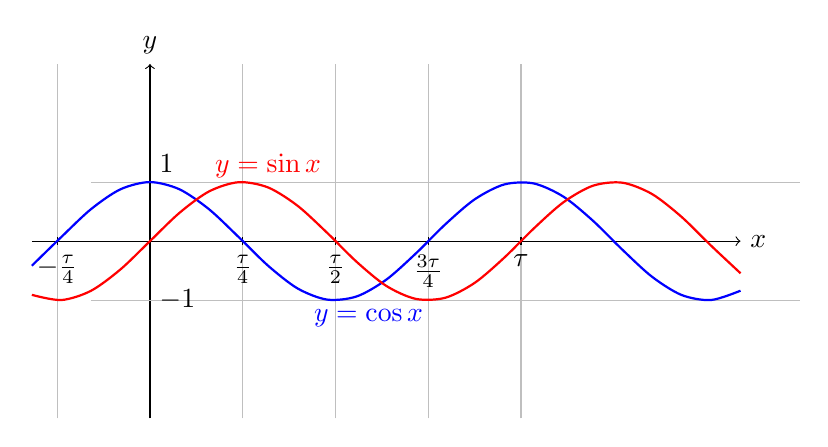
\begin{tikzpicture}[scale=0.75]
  \draw[->] (-2,0) -- (10,0) node[right] {$x$};
  \draw[->] (0,-3) -- (0,3) node[above] {$y$};
  \foreach \x/\xtext in
    {{pi/2}/{\frac \tau 4}, {pi}/{\frac \tau 2},
     {2*pi}/{\tau}, {3*pi/2}/{\frac {3\tau} 4}, {-pi/2}/{-\frac {\tau}{4}}} {
    \draw[shift={(\x,0)},lightgray] (0,-3) -- (0,3);
    \draw[shift={(\x,0)}] (0pt,2pt) -- (0pt,-2pt) node[below] {$\xtext$};
  }
  \foreach \y in {1, -1} {
    \draw[shift={(0,\y)},lightgray] (-1,0) -- (11,0);
  }
  \draw (0,1) node [above right] {$1$};
  \draw (0,-1) node [right] {$-1$};
  \draw[domain=-2:10,smooth,variable=\x,blue,thick] plot ({\x},{cos(deg(\x))});
  \draw[domain=-2:10,smooth,variable=\x,red,thick] plot ({\x},{sin(deg(\x))});
  \draw (3.7,-1) node[blue,below] {$y=\cos x$};
  \draw (2,0.9)  node[red,above] {$y=\sin x$};
  \end{tikzpicture}
  \caption{%
  I grafici delle funzioni $\sin$, $\cos$ di 
  un generico periodo $\tau$.}
\end{figure}

